% CVPR 2027 Paper Template; see https://github.com/cvpr-org/author-kit
% Style files (cvpr.sty, ieeenat_fullname.bst, preamble.tex) copied from author-kit-CVPR2027-v1-latex.zip.

\documentclass[10pt,twocolumn,letterpaper]{article}

%%%%%%%%% PAPER TYPE  - PLEASE UPDATE FOR FINAL VERSION
% \usepackage{cvpr}              % To produce the CAMERA-READY version
\usepackage[review]{cvpr}      % To produce the REVIEW version
% \usepackage[pagenumbers]{cvpr} % To force page numbers, e.g. for an arXiv version

% Local preview with Tectonic (XeTeX): cvpr.sty loads the Type 1 package times, which has no
% Unicode encoding; use the OpenType TeX Gyre clones instead. pdfLaTeX on Overleaf skips this block.
\ifdefined\XeTeXrevision
  \usepackage{fontspec}
  \setmainfont{texgyretermes}[Extension=.otf, UprightFont=*-regular, BoldFont=*-bold, ItalicFont=*-italic, BoldItalicFont=*-bolditalic]
  \setsansfont{texgyreheros}[Extension=.otf, UprightFont=*-regular, BoldFont=*-bold, ItalicFont=*-italic, BoldItalicFont=*-bolditalic]
  \setmonofont{texgyrecursor}[Extension=.otf, UprightFont=*-regular, BoldFont=*-bold, ItalicFont=*-italic, BoldItalicFont=*-bolditalic]
\fi

% Import additional packages in the preamble file, before hyperref
%% This file contains a number of tweaks that are typically applied to the main document.
%% They are not enabled by default, but can be enabled by uncommenting the relevant lines.

%%
%% Inline annotations; for predefined colors, refer to "dvipsnames" in the xcolor package:
%% https://tinyurl.com/overleaf-colors
%%
\newcommand{\red}[1]{{\color{red}#1}}
\newcommand{\todo}[1]{{\color{red}#1}}
\newcommand{\TODO}[1]{\textbf{\color{red}[TODO: #1]}}
%%
%% disable for camera ready / submission by uncommenting these lines  
%%
% \renewcommand{\TODO}[1]{}
% \renewcommand{\todo}[1]{#1}

%%
%% work harder in optimizing text layout. Typically shrinks text by 1/6 of page, enable
%% it at the very end of the writing process, when you are just above the page limit
%%
% \usepackage{microtype}

%%
%% fine-tune paragraph spacing
%%
% \renewcommand{\paragraph}[1]{\vspace{.5em}\noindent\textbf{#1.}}

%%
%% globally adjusts space between figure and caption
%%
% \setlength{\abovecaptionskip}{.5em}


%%
%% Allows "the use of \paper to refer to the project name"
%% with automatic management of space at the end of the word
%%
% \usepackage{xspace}
% \newcommand{\paper}{ProjectName\xspace}

%%
%% Commonly used math definitions
%%
% \DeclareMathOperator*{\argmin}{arg\,min}
% \DeclareMathOperator*{\argmax}{arg\,max}

%%
%% Tigthen underline
%%
% \usepackage{soul}
% \setuldepth{foobar}
% Two-column teaser (fig/teaser.tex); the CVPR 2027 preamble no longer loads these packages.
\usepackage{cuted}
\usepackage{currfile}
\usepackage{caption}
\newcommand{\NUM}{\textbf{\color{red}[NUM]}}

\definecolor{cvprblue}{rgb}{0.21,0.49,0.74}
\usepackage[pagebackref,breaklinks,colorlinks,allcolors=cvprblue]{hyperref}

\def\confName{CVPR}
\def\confYear{2027}

%%%%%%%%% TITLE
\title{Color-Mapping Immunization: Purification-Robust Protection of Images against Diffusion-Based Editing}

%%%%%%%%% AUTHORS
\author{First Author\\
Institution1\\
{\tt\small firstauthor@i1.org}
}

\begin{document}
\maketitle
\begin{strip}
\centering
\includegraphics[width=.24\linewidth]{example-image-a}\hfill
\includegraphics[width=.24\linewidth]{example-image-b}\hfill
\includegraphics[width=.24\linewidth]{example-image-c}\hfill
\includegraphics[width=.24\linewidth]{example-image-a}
\captionsetup{hypcap=false}
\captionof{figure}{\TODO{Teaser draft pending: original $\rightarrow$ protected $\rightarrow$ purified $\rightarrow$ edited, for an additive defense and for color-mapping immunization at matched distortion, with the undefended edit as reference.}}
\captionsetup{hypcap=true}
\label{fig:teaser}%
\end{strip}

\begin{abstract}
Recent generative image models such as Stable Diffusion allow a publicly released photograph, portraits in particular, to be modified with a text prompt, which raises privacy and security concerns. Image immunization addresses this threat by modifying a photograph before its release. Most existing methods superimpose an additive adversarial perturbation on the image, which reduces the chance that an edit succeeds. The energy of this perturbation lies mainly at high spatial frequencies. Purification operations such as JPEG compression, Gaussian blurring, and encoder-based reconstruction therefore remove it with little effort. This vulnerability stems from the spatial structure of the perturbation. We propose color-mapping immunization, a filter-like defense that encodes the protection in the colors of the image. Each image receives its own 3D color lookup table (LUT), the operator of global color grading. Acting on colors alone, the LUT introduces no spatial structure into the image, and the protection it carries persists through purification. The protected image appears as a color-graded version of the original. On InstructPix2Pix at matched distortion, the edit displacement retained after purification, averaged over all purification methods, is \NUM{} times that of additive defenses.
\end{abstract}

\section{Introduction}
\label{sec:intro}

% P1: background and the development of immunization
Recent generative image models such as Stable Diffusion~\cite{rombach2022ldm} and the instruction-guided editors built on them~\cite{brooks2023instructpix2pix,zhao2024ultraedit,flux2025kontext} allow a publicly released photograph, portraits in particular, to be modified with a text prompt. This capability raises privacy and security concerns. Image immunization~\cite{salman2023photoguard} addresses them on the side of the image owner, who modifies a photograph before release so that edits of the released copy diverge from edits of the original. PhotoGuard introduced this setting for Stable Diffusion image-to-image editing and inpainting. Subsequent work extended it to instruction-guided editing~\cite{chen2024editshield,dctshield2025}, inpainting under attacker-chosen masks~\cite{diffusionguard2025,dia2025}, facial identity~\cite{wang2025facelock}, and diffusion-transformer editors~\cite{decontext2025,nulledit2026}, and replaced per-image optimization with a trained feed-forward generator~\cite{diffvax2026}.

% P2: common form of existing methods
Most of these methods share one form. They superimpose an additive adversarial perturbation $\delta$ on the image, optimized under an $\ell_\infty$ or $\ell_2$ budget with projected gradient descent against a component of the editor~\cite{salman2023photoguard,liang2023mist,chen2024editshield,dia2025,dctshield2025}. The perturbation is set independently at each pixel and forms a pattern tied to the pixel grid of the original photograph, with most of its energy at high spatial frequencies \TODO{radial power spectrum of $\delta$, supplementary}. Methods designed for robustness keep the additive form and change where $\delta$ is placed. DCT-Shield~\cite{dctshield2025} perturbs quantized JPEG coefficients, and BlurGuard~\cite{blurguard2025} applies region-wise Gaussian blur to $\delta$ to bring its spectrum closer to that of natural images.

% P3: findings of purification studies
This spatial structure makes the perturbation fragile. Purification operations that an attacker can apply before editing remove it. JPEG compression~\cite{sandoval2023jpeg} and noisy upscaling~\cite{honig2025noisyupscaling} bypass several protections, and VAE-based purification removes the protection of six methods without access to the protected images or to the defense~\cite{purifyonce2026}. Contrastive adversarial training of a lightweight adapter removes it on the side of the editor~\cite{cat2025}. Evaluations of edit outcomes report that protected images are often still edited as instructed~\cite{icip2025disruptive} and that protections fail under chains of common transformations~\cite{doprotect2026}. H\"{o}nig~\etal~\cite{honig2025noisyupscaling} attribute this to a structural disadvantage of the defender, whose protection is fixed before the attacker selects a purification.

% P4: the proposed carrier
We propose color-mapping immunization, a filter-like defense that encodes the protection in the colors of the image. Each image receives its own 3D color lookup table (LUT), the operator of global color grading~\cite{zeng2020lut}. Acting on colors alone, the LUT introduces no spatial structure into the image, and the protection it carries persists through purification (\cref{sec:carrier}). The protected image appears as a color-graded version of the original (\cref{fig:teaser}). Color mappings have served as adversarial carriers against image classifiers~\cite{laidlaw2019functional,zhao2023advcf,yuan2022ncf}. We bring this family of transformations to immunization against diffusion editing.

% P5: naturalness by parameterization
A LUT optimized without restriction can produce banding, unnatural skin tones, and colored fringes in neutral regions. Adding a penalty for each such artifact leads to constraints that conflict during optimization (\cref{sec:exp_ablation}). We instead restrict the form of the mapping. The LUT rotates each color vector about the black point, with the gray axis as the polar axis. The polar angle, which governs saturation, and the azimuth, which governs hue, each change within a small bound, and the rotation varies smoothly across color space (\cref{sec:feasible}). Every mapping in this family is a mild, smooth color shift, so the optimization needs no penalty terms or projection and maximizes the defense objective alone.

% P6: comparison protocol
Defenses of different forms are compared at matched distortion. We measure defense distortion as the LPIPS between the protected and the original image, and edit displacement as the LPIPS between the edits of the two. The operating points of additive methods and of color mappings lie close to one line on these axes, and adjusting the budget of a method moves it along that line (\cref{fig:plane}). At equal distortion the defenses are therefore comparable before purification, and we evaluate how much of their displacement remains after it (\cref{sec:exp_purify}).

% P7: measurement of naturalness
Reference-based quality metrics and preference models count a change of tone as degradation, and PieAPP, TOPIQ-FR, and HPSv3 rank a color-graded photograph below an additive perturbation of the same LPIPS (\cref{sec:exp_percept}). We report these metrics together with a color-aligned distortion that factors out the best-fitting global color transform before comparison, a reference band of common grading presets, and a user study.

Our contributions are:
\begin{itemize}
  \item We propose color-mapping immunization, a filter-like defense that protects each image with its own 3D LUT and introduces no spatial structure into the image.
  \item On InstructPix2Pix at matched distortion, the edit displacement our defense retains after purification, averaged over all purification methods, is \NUM{} times that of additive defenses.
  \item We propose an evaluation of naturalness for tone-changing defenses that combines color-aligned distortion, a reference band of grading presets, and a user study.
\end{itemize}

\section{Related Work}
\label{sec:related}

\begin{figure*}[t]
  \centering
  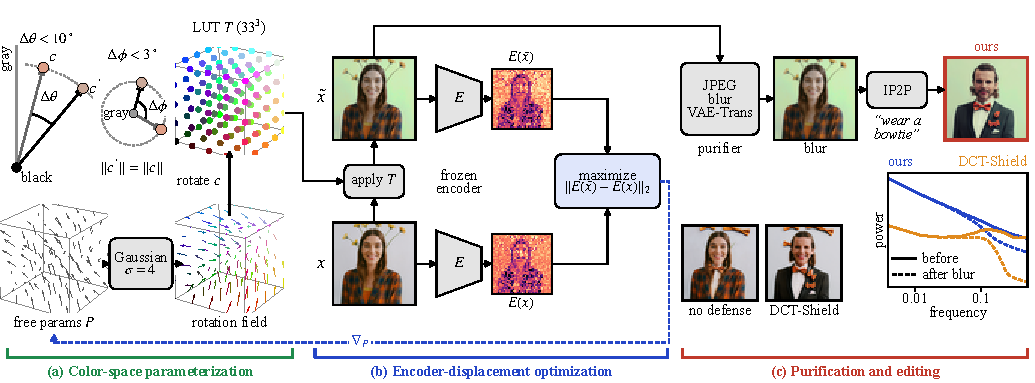
\includegraphics[width=\linewidth]{fig/method_overview.pdf}
  \caption{Overview of color-mapping immunization. (a)~Free parameters $P$ on a $33^3$ grid are smoothed by a Gaussian kernel ($\sigma = 4$ grid cells) into a rotation field. The field rotates each color vector $c$ about the black point and preserves $\|c\|$. With the gray axis as the polar axis, the polar angle changes by less than $10^\circ$ and the azimuth by less than $3^\circ$ before clipping to the RGB gamut; the angles in the sketch are enlarged. (b)~The resulting LUT $T$ is applied to the image $x$, and $P$ is optimized to maximize the displacement $\|E(\tilde{x}) - E(x)\|_2$ of the frozen VAE encoder $E$. (c)~The attacker purifies the protected image $\tilde{x}$ (here Gaussian blur, $\sigma = 2$) and edits it with InstructPix2Pix (``Let the person wear a bowtie''). The edit of our protected image replaces the person; after the same blur, the DCT-Shield~\cite{dctshield2025} protection keeps the person and changes only the clothing. ``No defense'' is the edit of the unprotected original. The spectra show the perturbation power averaged over eight portraits before (solid) and after (dashed) blur, each on its own unlabeled vertical scale.}
  \label{fig:overview}
\end{figure*}

\paragraph{Immunization against diffusion editing.}
PhotoGuard~\cite{salman2023photoguard} introduced protection against Stable Diffusion editing with an encoder attack and a costlier diffusion attack. Later methods kept the additive form and changed the target or the budget. Mist and AdvDM~\cite{liang2023mist,liang2023advdm} combine a textural loss on the encoder with a semantic loss on the denoiser. EditShield~\cite{chen2024editshield} targets instruction-guided editing, DIA~\cite{dia2025} attacks the inversion trajectory of inpainting, FaceLock~\cite{wang2025facelock} protects facial identity, and DiffVax~\cite{diffvax2026} replaces per-image optimization with a trained feed-forward network. \TODO{SIFM, DANP, DAYN.} Protections for DiT editors~\cite{decontext2025,nulledit2026} also use additive perturbations. Robustness-oriented variants change where the perturbation is placed. DCT-Shield~\cite{dctshield2025} perturbs JPEG coefficients, DiffusionGuard~\cite{diffusionguard2025} targets the early denoising steps, and BlurGuard~\cite{blurguard2025} applies region-wise blur to the noise. In every case the protection remains an additive pattern on the pixel grid, which is the component that blurring, compression, and reconstruction attenuate. We keep the threat model of this line of work and replace the carrier.

\paragraph{Purification.}
Simple operations remove protective perturbations. JPEG compression~\cite{sandoval2023jpeg} and noisy upscaling~\cite{honig2025noisyupscaling} bypass several protections, and H\"{o}nig~\etal~\cite{honig2025noisyupscaling} argue that the defender is structurally disadvantaged because the protection must be fixed before the attacker chooses a purification. VAE-based purifiers remove the protection of six methods without knowledge of how the images were protected~\cite{purifyonce2026}, and CAT~\cite{cat2025} removes it by fine-tuning a small adapter. Other studies find that edits of protected images often still follow the prompt~\cite{icip2025disruptive} and that protections fail under chains of common transformations~\cite{doprotect2026}. These works establish that additive protections can be removed, and they evaluate each protection at its own budget. We adopt the image-space purifications of this literature as part of the evaluation and compare all defenses at matched distortion.

\paragraph{Color-based adversarial examples.}
Adversarial examples for image classifiers need not be additive noise. Hue and saturation shifts~\cite{hosseini2018semantic}, per-image color lookup tables~\cite{laidlaw2019functional}, piecewise-linear color filters~\cite{zhao2020ace,zhao2023advcf}, and semantic recoloring~\cite{shamsabadi2020colorfool,bhattad2020cadv} all cause misclassification. Natural Color Fool~\cite{yuan2022ncf} restricts colors to distributions observed in real images, and AdvCF~\cite{zhao2023advcf} found color filters more robust than noise to JPEG and filtering. These attacks target classifiers and bound the color change with $\ell_p$ radii on the table or with semantic color ranges, which assume a classification decision as the outcome. We take the per-image lookup table of ReColorAdv~\cite{laidlaw2019functional} as the carrier, apply it to immunization against diffusion editing, and bound it with a smooth rotation of saturation and hue (\cref{sec:feasible}).

\paragraph{Judging color changes.}
LPIPS and DISTS~\cite{zhang2018lpips,ding2020dists} compare deep features of an image and its reference, and CIEDE2000~\cite{sharma2005ciede2000} compares colors pixel by pixel. S-CIELAB~\cite{zhang1997scielab} adds spatial filtering that models color acuity, CD-Flow~\cite{chen2023cdflow} learns a color difference for photographs, and the measure of Rajashekar~\etal~\cite{rajashekar2010color} tolerates changes of illumination. Preference models~\cite{kirstain2023pickscore,ma2025hpsv3} score an image against a text prompt, and SCOOTER~\cite{scooter2025} provides a protocol for human studies of unrestricted adversarial examples. Reference-based measures, including PSNR and SSIM, count a global change of tone as error and therefore rank a color-graded image below additive noise of equal LPIPS. We report LPIPS as the common distortion axis, add no-reference aesthetic scores, and follow the principle of~\cite{rajashekar2010color} with a color-aligned distortion that factors out the best-fitting global color transform before comparison.

\section{Method}
\label{sec:method}


\Cref{fig:overview} summarizes the method. The defense is a per-image 3D LUT (\cref{sec:carrier}) whose form is restricted to smooth rotations of color (\cref{sec:feasible}), optimized against the VAE encoder of the editor (\cref{sec:objective}).

\subsection{Threat model}
\label{sec:threat}
The defender processes an image $x$ before sharing it and publishes $\tilde{x}$. The attacker edits $\tilde{x}$ with a public editor $E(\cdot, p)$ and an instruction $p$, possibly after applying a purification $P$. We assume the defender knows the editor's weights but cannot change them, and does not know $p$. During optimization the defender uses no instruction. We measure success by edit displacement, the LPIPS distance between $E(P(\tilde{x}), p)$ and $E(P(x), p)$.

\subsection{A color lookup table as the carrier}
\label{sec:carrier}
We parameterize the defense as a 3D LUT $T : [0,1]^3 \to [0,1]^3$ with $33^3$ lattice nodes. Each pixel is mapped by trilinear interpolation, $\tilde{x}_i = T(x_i)$. Two pixels of the same color therefore receive the same output, and the defense has no spatial structure of its own. \TODO{A short argument for why purification operators that preserve content approximately commute with $T$, while they do not preserve $\delta$ in $x + \delta$.}

\subsection{Smooth color rotations}
\label{sec:feasible}
A LUT optimized without restriction produces color bands, unnatural skin tones, and colored fringes in neutral regions. We restrict $T$ to rotations of color about the black point. Each lattice color $c \in [0,1]^3$ is treated as a vector with direction $\hat{c} = c / \|c\|$, and the gray axis $g = (1,1,1)/\sqrt{3}$ serves as the polar axis. The polar angle of $\hat{c}$, its deviation from $g$, governs saturation, and its azimuth around $g$ governs hue.

\paragraph{Rotation field.} The free parameters $P \in \mathbb{R}^{3 \times 33^3}$ assign a vector to every lattice node. A separable 3D Gaussian filter with $\sigma = 4$ lattice cells, truncated at $3\sigma$ and applied with replicated borders, turns them into a smooth field $V = G_\sigma * P$, so that neighboring colors rotate by similar amounts. At each node, the component of $V$ along $\hat{c}$ is removed, and the remainder is split into a meridian component $v_p$, which lies in the plane spanned by $\hat{c}$ and $g$, and an azimuthal component $v_h$ along $h = g \times \hat{c} / \|g \times \hat{c}\|$.

\paragraph{Bounded rotation.} The two components rotate $\hat{c}$ in turn, each through a $\tanh$ saturation that bounds the angle without clipping:
\begin{align}
  d &= \hat{c} + \frac{v_p}{\|v_p\|}\, \tan\theta_{\max} \tanh\!\Big(\frac{\|v_p\|}{\tan\theta_{\max}}\Big), \\
  o &= d + b \tanh\!\Big(\frac{v_h}{b}\Big)\, \frac{g \times d}{\|g \times d\|}, \qquad b = \tan\phi_{\max}\, \|g \times d\|, \\
  T(c) &= \mathrm{clip}_{[0,1]}\big(\|c\|\, o / \|o\|\big).
  \label{eq:rotation}
\end{align}
The first step changes the polar angle by less than $\theta_{\max}$ and the second changes the azimuth by less than $\phi_{\max}$; on the gray axis $b = 0$ and the hue of neutral colors is not defined. We use $\theta_{\max} = 10^\circ$ and $\phi_{\max} = 3^\circ$, so hue changes less than saturation. The output keeps the magnitude $\|c\|$, and the bounds hold before the final per-channel clipping to the RGB gamut. Pixels are mapped by trilinear interpolation of the $33^3$ node outputs.

Every mapping in this family is a smooth change of saturation and hue at fixed vector magnitude. Naturalness is thus a property of the parameterization, and the optimization needs no penalty terms, projection, or bound on distortion. An earlier version added one penalty for each observed artifact and solved the problem with an augmented Lagrangian; the penalties pulled in different directions, and on one image only 1 of 180 checkpoints satisfied all of them (\cref{sec:exp_ablation}).

\subsection{Objective}
\label{sec:objective}
We push the editor's VAE latent away from that of the original. With $\mu_\mathcal{E}$ the posterior mean of the VAE encoder, the objective is the mean squared difference over all $n$ latent elements,
\begin{equation}
  \max_P \; \frac{1}{n} \big\| \mu_\mathcal{E}(T_P(x)) - \mu_\mathcal{E}(x) \big\|_2^2 .
  \label{eq:objective}
\end{equation}
This needs one forward pass through the encoder and no instruction. The method also needs gradients only through the VAE, which matters for large editors such as FLUX.1 Kontext, whose 12B transformer we never back-propagate through. Other objectives are compared in \cref{sec:exp_ablation}.

\subsection{Optimization}
\label{sec:optimization}
We initialize $P$ with independent Gaussian entries of standard deviation 0.002 and optimize \cref{eq:objective} with Adam ($\beta_1 = 0.5$, $\beta_2 = 0.99$) for 1800 steps at $512^2$ resolution. The learning rate follows a cosine decay from $3 \times 10^{-4}$ to $10^{-5}$ over the first two thirds of the steps and stays at $10^{-5}$ afterwards. The protected image of the final step is delivered as an 8-bit PNG. Solving one image takes 8.5 to 9 minutes on a single RTX 3090.

\section{Experiments}
\label{sec:exp}

We compare color-mapping immunization with eleven additive defenses. After the setup in \cref{sec:exp_setup}, \cref{sec:exp_anti} reports the main result, the edit displacement that remains after purification at matched distortion. \Cref{sec:exp_plane} places all defenses on the distortion--displacement plane before purification and lists their native budgets, and \cref{sec:exp_purify} measures how much of each perturbation purification removes. We then evaluate other editors in \cref{sec:exp_gen} and the perceptual quality of the protected images in \cref{sec:exp_percept}, and conclude with ablations in \cref{sec:exp_ablation}.

\subsection{Setup}
\label{sec:exp_setup}
\paragraph{Data.} Eight $512^2$ portraits with subject masks. \TODO{Portraits from Pexels, $N = 306$ to $500$.}
\paragraph{Attack.} InstructPix2Pix~\cite{brooks2023instructpix2pix} with Euler-Ancestral sampling (50 steps, text guidance 7.5, image guidance 1.8, seed 20260812) and the four accessory instructions of FaceLock~\cite{wang2025facelock}, giving $8 \times 4 = 32$ edits per method.
\paragraph{Purification.} Seven standard operations: JPEG at quality 80, 50, and 30; Gaussian blur with $\sigma = 1$ and $2$; a 10\% crop followed by resizing; and a $15^\circ$ rotation. VAE-Trans~\cite{purifyonce2026}, a fine-tuned VAE encoder used as a purifier, is reported separately.
\paragraph{Baselines.} Eleven additive methods. Each is rescaled to a common defense LPIPS (the matched-distortion arm, defense LPIPS 0.300--0.374) and also run at its native budget. DiffVax~\cite{diffvax2026} has no budget to rescale and appears only in the native-budget comparison.
\paragraph{Metrics.} Defense distortion is the LPIPS between the protected and the original image; we add no-reference aesthetic scores, which do not use the original as a reference. Edit displacement is the LPIPS between the edits of the protected and the undefended image, with SigLIP image similarity as a semantic counterpart. Retention is the per-edit ratio of displacement after and before purification, averaged over edits. Pixel-wise and structural references such as PSNR, SSIM, and DISTS count a global change of tone as error; we report them in the supplementary material.

\subsection{Robustness to purification}
\label{sec:exp_anti}
\Cref{tab:main} compares all defenses at matched distortion after purification. Before purification, the additive methods displace edits by 0.29--0.44 LPIPS and ours by 0.374. Averaged over the seven purifications, their displacement falls to 0.13--0.24, while ours stays at 0.367 with a retention of 1.02. Under the strongest operation for each additive method, Gaussian blur with $\sigma = 2$, their displacement drops to 0.04--0.15; our lowest purification, crop-and-resize, leaves 0.339. After VAE-Trans, our defense keeps 0.301 against 0.02--0.07 for the additive methods. Our defense reaches these values at a defense LPIPS of 0.296, below every additive arm, and with a LAION aesthetic score equal to that of the original. \Cref{fig:purified_plane} places each defense by its defense LPIPS and its displacement after purification.

\begin{table*}[t]
  \centering
  \small
  \setlength{\tabcolsep}{4pt}
  \begin{tabular}{lcc|cccc|c|cc}
    \toprule
    & \multicolumn{2}{c|}{Defense image} & \multicolumn{4}{c|}{Edit LPIPS $\uparrow$} & & \multicolumn{2}{c}{SigLIP sim.\ $\downarrow$} \\
    Method & LPIPS & LAION & None & 7-mean & Lowest & VAE-Trans & Retention & None & 7-mean \\
    \midrule
    Original & -- & 5.478 & & & & & & & \\
    \midrule
    DAYN & .328 & 5.527 & .386 & .241 & .148 & .067 & .639 & .884 & .931 \\
    DIA-R & .348 & 5.623 & .390 & .229 & .105 & .055 & .603 & .872 & .943 \\
    DIA-PT & .327 & 5.428 & .386 & .216 & .099 & .048 & .579 & .880 & .946 \\
    SIFM & .300 & 5.561 & .380 & .201 & .091 & .049 & .546 & .885 & .953 \\
    DANP & .308 & 5.516 & .370 & .200 & .086 & .050 & .554 & .899 & .957 \\
    Mist & .367 & 5.556 & .400 & .185 & .057 & .037 & .465 & .932 & .976 \\
    PhotoGuard-Enc & .367 & 5.566 & .438 & .179 & .059 & .040 & .420 & -- & -- \\
    PhotoGuard-$\ell_\infty$ & .374 & 5.564 & .337 & .177 & .057 & .039 & .532 & .951 & .976 \\
    PhotoGuard-$\ell_2$ & .323 & 5.518 & .322 & .164 & .045 & .022 & .513 & .924 & .962 \\
    DCT-Shield & .326 & 5.564 & .322 & .129 & .037 & .030 & .408 & .901 & .970 \\
    DCT-Shield-Y & .315 & 5.418 & .291 & .128 & .041 & .034 & .451 & .923 & .969 \\
    \midrule
    Ours & .296 & 5.482 & .374 & \textbf{.367} & \textbf{.339} & \textbf{.301} & \textbf{1.020} & .874 & \textbf{.883} \\
    \bottomrule
  \end{tabular}
  \caption{Main comparison at matched distortion on InstructPix2Pix (8 portraits $\times$ 4 instructions, seed 20260812). Defense image: LPIPS to the original and LAION aesthetic score. Edit LPIPS between the edits of the protected and the undefended image: before purification (None), averaged over the seven standard purifications (7-mean), under the purification with the lowest mean (Lowest; Gaussian blur $\sigma = 2$ for every additive method, crop-and-resize for ours), and after VAE-Trans. SigLIP was not measured for PhotoGuard-Enc. Retention: per-edit ratio of purified to unpurified displacement, averaged over the seven purifications. SigLIP sim.: image similarity between the two edits.}
  \label{tab:main}
\end{table*}

\begin{figure}[t]
  \centering
  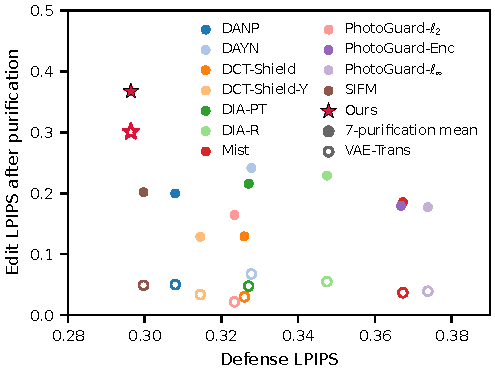
\includegraphics[width=\linewidth]{fig/purified_plane.pdf}
  \caption{Defense LPIPS versus edit LPIPS after purification at matched distortion on InstructPix2Pix (8 portraits $\times$ 4 instructions). Filled markers: mean over the seven standard purifications; open markers: after VAE-Trans.}
  \label{fig:purified_plane}
\end{figure}

\subsection{Without purification: one line for all methods}
\label{sec:exp_plane}
\Cref{fig:plane} plots edit displacement before purification against defense LPIPS for every method, including budget sweeps for six of them. The 34 points of the additive methods fit edit LPIPS $= 0.871 \times$ defense LPIPS $+ 0.072$ with $r = 0.955$, and each swept method stays on its own straight line ($r = 0.987$ to $1.000$). With DISTS or PieAPP on the horizontal axis, each method is still close to linear ($r = 0.87$ to $0.99$), but the slopes differ between methods. Our defense lies 0.044 above the pooled LPIPS line. Before purification, the color mapping and the additive methods are thus comparable at equal distortion. \Cref{tab:native} lists the methods at their native budgets, where defense LPIPS ranges from 0.043 to 0.666 and the ranking of displacement follows the ranking of distortion.

\begin{figure}[t]
  \centering
  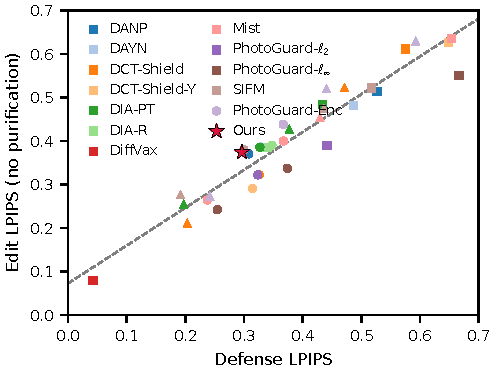
\includegraphics[width=\linewidth]{fig/plane.pdf}
  \caption{Defense LPIPS versus edit LPIPS before purification on InstructPix2Pix (8 portraits $\times$ 4 instructions). Squares: native budgets; circles: matched-distortion arm; triangles: budget sweeps. The dashed line is the least-squares fit to the 34 additive points ($r = 0.955$).}
  \label{fig:plane}
\end{figure}

\begin{table}[t]
  \centering
  \small
  \setlength{\tabcolsep}{3pt}
  \begin{tabular}{lccccc}
    \toprule
    & & \multicolumn{3}{c}{Edit LPIPS} & \\
    Method & Def. & None & 7-mean & Lowest & Ret. \\
    \midrule
    Mist & .654 & .636 & .503 & .379 & .793 \\
    PhotoGuard-$\ell_\infty$ & .666 & .551 & .461 & .322 & .843 \\
    DANP & .527 & .514 & .409 & .291 & .809 \\
    SIFM & .517 & .522 & .392 & .300 & .767 \\
    DCT-Shield-Y & .648 & .626 & .366 & .136 & .593 \\
    DAYN & .487 & .481 & .364 & .267 & .776 \\
    DIA-PT & .433 & .483 & .308 & .191 & .648 \\
    DCT-Shield & .575 & .611 & .261 & .131 & .435 \\
    PhotoGuard-$\ell_2$ & .442 & .390 & .255 & .123 & .658 \\
    DIA-R & .339 & .386 & .226 & .108 & .600 \\
    DiffVax & .043 & .079 & .081 & .065 & 1.059 \\
    \midrule
    Ours & .296 & .374 & .367 & .339 & 1.020 \\
    \bottomrule
  \end{tabular}
  \caption{Native budgets on InstructPix2Pix (8 portraits $\times$ 4 instructions). Def.: defense LPIPS; Ret.: retention over the seven purifications. Lowest is Gaussian blur $\sigma = 2$ except for DiffVax ($\sigma = 1$) and ours (crop-and-resize). PhotoGuard-Enc has no native-budget run.}
  \label{tab:native}
\end{table}

\subsection{What purification removes}
\label{sec:exp_purify}
To see what a purifier $P$ does to the defense itself, before any editing, we compute the fraction of the perturbation that survives, $\mathrm{LPIPS}(P(\tilde{x}), P(x)) / \mathrm{LPIPS}(\tilde{x}, x)$. \Cref{tab:survival} shows the result. Geometric operations (crop-resize, rotation) leave most perturbations in place for every method. JPEG, blur, and VAE purification are where the methods separate. Strong blur leaves 5--22\% of an additive perturbation and VAE purification leaves 2--9\%, while a LUT keeps most of its change because the colors of the photo survive these operations.

\begin{table}[t]
  \centering
  \small
  \setlength{\tabcolsep}{3.5pt}
  \begin{tabular}{lccccc}
    \toprule
    Method & Def. & 7-mean & JPEG30 & Blur2 & VAE \\
    \midrule
    DAYN & .328 & .535 & .398 & .219 & .092 \\
    DIA-R & .348 & .515 & .337 & .167 & .071 \\
    DANP & .308 & .483 & .317 & .167 & .070 \\
    DIA-PT & .327 & .473 & .295 & .130 & .059 \\
    SIFM & .300 & .467 & .303 & .143 & .053 \\
    PhotoGuard-$\ell_\infty$ & .374 & .387 & .205 & .088 & .034 \\
    Mist & .367 & .382 & .216 & .088 & .038 \\
    PhotoGuard-$\ell_2$ & .323 & .377 & .180 & .071 & .019 \\
    PhotoGuard-Enc & .367 & .373 & .202 & .101 & .039 \\
    DCT-Shield-Y & .315 & .312 & .209 & .057 & .038 \\
    DCT-Shield & .326 & .288 & .123 & .048 & .027 \\
    \midrule
    Penalty LUT (ablation) & .287 & .838 & .858 & .693 & .457 \\
    Ours & \NUM & \NUM & \NUM & \NUM & \NUM \\
    \bottomrule
  \end{tabular}
  \caption{Fraction of the perturbation that survives purification, $\mathrm{LPIPS}(P(\tilde{x}), P(x)) / \mathrm{LPIPS}(\tilde{x}, x)$, averaged over 8 images. Def.: defense LPIPS; 7-mean: mean over the seven standard purifications.}
  \label{tab:survival}
\end{table}

We then vary the strength of each purifier and edit the purified images (\cref{tab:strength}). For the additive methods, edit displacement falls steadily as JPEG quality drops or blur grows, reaching 0.03--0.14 at the strongest settings. For reference, editing the same undefended image with two different seeds already gives 0.109. The penalty-based LUT (ablation) stays between 0.25 and 0.34 over the whole range, and JPEG compression barely affects it.

\begin{table}[t]
  \centering
  \small
  \setlength{\tabcolsep}{3pt}
  \begin{tabular}{lcccccc}
    \toprule
    & \multicolumn{2}{c}{JPEG quality} & \multicolumn{2}{c}{Blur $\sigma$} & \multicolumn{2}{c}{Resize} \\
    Method & 95 & 10 & 0.5 & 3 & 0.75 & 0.25 \\
    \midrule
    DIA-PT & .336 & .135 & .334 & .044 & .277 & .108 \\
    Mist & .306 & .138 & .324 & .039 & .239 & .083 \\
    PhotoGuard-Enc & .289 & .129 & .311 & .040 & .221 & .086 \\
    DCT-Shield & .072 & .087 & .229 & .033 & .142 & .042 \\
    Penalty LUT (ablation) & .339 & .340 & .325 & .245 & .310 & .276 \\
    Ours & \NUM & \NUM & \NUM & \NUM & \NUM & \NUM \\
    \bottomrule
  \end{tabular}
  \caption{Edit displacement (LPIPS) after purification at increasing strength; 8 images $\times$ 4 instructions, InstructPix2Pix, matched distortion.}
  \label{tab:strength}
\end{table}

\TODO{Note on DCT-Shield, whose displacement is low already at JPEG quality 95 and does not decrease monotonically with strength.}

A matched random LUT also survives purification (0.196 after VAE-Trans), which tells us that the robustness comes from the carrier. Optimization adds the strength: within the same family, optimized mappings displace edits 32--61\% more than random ones at equal distortion.

\subsection{Other editors}
\label{sec:exp_gen}
InstructPix2Pix, SD inpainting, and SD 2.1 share the same VAE encoder weights, so a defense computed for one of them targets all three. On SD inpainting the penalty-based LUT gives 0.343 before purification, 0.288--0.323 under the seven purifications, and 0.241 after VAE-Trans, close to its InstructPix2Pix numbers. FLUX.1 Kontext~\cite{flux2025kontext} and UltraEdit~\cite{zhao2024ultraedit}, which builds on SD3, have their own 16-channel VAEs. Defenses computed on InstructPix2Pix and evaluated on these two editors keep the ranking of methods (Spearman 0.951). \TODO{Per-encoder results: ours optimized on the FLUX and SD3 encoders; baselines that can be ported with their own losses (PhotoGuard encoder attack, DCT-Shield, DCT-Shield-Y, and the textural term of Mist).}

\subsection{Is the result still a good photo?}
\label{sec:exp_percept}
Our defenses change the colors of the image on purpose, so we do not expect them to score well on metrics that compare against the original. They do not. PieAPP, TOPIQ-FR, AHIQ, CKDN, CW-SSIM, NLPD, GMSD, and MS-SSIM all rank the LUT defenses below the additive ones, and so do PickScore~\cite{kirstain2023pickscore} and HPSv3~\cite{ma2025hpsv3}. These numbers mix two things: the change of tone, which is intended and visible, and any damage to the image, which is not intended.

To separate them, we fit a global color transform from each defended image back to the original and measure what remains. With a smooth $9^3$ LUT as the transform, the penalty-based LUT drops from 0.287 to 0.137 LPIPS, below every additive method (0.282--0.358), and its DISTS, PieAPP, and SSIM fall inside the additive range. With a simpler affine transform in Lab, LPIPS drops to 0.209 but DISTS and PieAPP stay above the additive methods. Since aligning a LUT with a LUT may look circular, we apply the same alignment to twenty color-grading presets~\cite{rawtherapee_haldclut}. Film presets align almost perfectly (0.010--0.043), while some creative presets do not (bleach bypass stays at 0.340). Before alignment, the penalty-based LUT changes the image about as much as a creative preset (LPIPS 0.287 against 0.061--0.353) and more than a film preset (0.031--0.115).

No-reference scores tell a similar story. Relative to the original, the LAION aesthetic score of the penalty-based LUT rises by 0.175 (additive methods: $-0.061$ to $+0.145$), and MUSIQ, CLIP-IQA, and ImageReward fall by amounts inside the additive range. \TODO{User study: two-alternative naturalness judgments and edited-or-not detection following~\cite{scooter2025}; final numbers for our method.}

\subsection{Ablations}
\label{sec:exp_ablation}
\Cref{tab:ablation} lists the ablations. The first row compares ways of keeping the mapping natural, from per-artifact penalties solved with an augmented Lagrangian to the rotation parameterization of \cref{sec:feasible}.

\begin{table}[t]
  \centering
  \small
  \setlength{\tabcolsep}{3pt}
  \begin{tabular}{ll}
    \toprule
    Axis & Variants \\
    \midrule
    Naturalness & per-artifact penalties / single-constant bounds / feasible set / rotation (ours) \\
    Rotation & single angle bound / separate saturation and hue bounds \\
    Carrier & RGB curves / $(a^*, b^*)$ warp / LUT $17^3$, $33^3$ \\
    Objective & encoder latent / equivariance / implicit classifier \\
    Control & random LUT and random filter, matched distortion \\
    \bottomrule
  \end{tabular}
  \caption{Ablation axes. \TODO{numbers}}
  \label{tab:ablation}
\end{table}

\section{Limitations}
\label{sec:discussion}
A large edit displacement does not always mean a failed edit. At the matched-distortion point, in 19 of the 32 cells the requested accessory still appears for every method, ours included; displacement measures how far the edit moves, not whether the attacker gets what they asked for. We do not evaluate attackers that estimate and undo a global color mapping, for example with an image-adaptive LUT enhancement network~\cite{zeng2020lut} or with color normalization, and such an attacker is the natural next test for this kind of defense. Our defenses are also visible: the photo looks regraded, and we can only argue, with the measurements in \cref{sec:exp_percept}, that it looks like a regraded photo rather than a damaged one. Finally, optimizing one LUT takes 12 to 25 minutes per image on an RTX 3090. The universal LUT removes this cost at some loss of strength.

\section{Conclusion}
\label{sec:conclusion}
\TODO{Conclusion, written after the final results.}

\section*{LLM Usage Statement}
\TODO{Required by the CVPR 2027 guidelines; does not count toward the page limit. Name the tools, the affected parts (text, figures, code, experiments, related work), and the extent of use, without revealing authorship.}

{
    \small
    \bibliographystyle{ieeenat_fullname}
    \bibliography{main}
}

% WARNING: do not forget to delete the supplementary pages from your submission
% \clearpage
\setcounter{page}{1}
\maketitlesupplementary

\section{Protocol details}
\TODO{Data, masks, prompts, purification parameters, seeds, matched-distortion rescaling.}

\section{Baseline provenance and budget conversion}
\TODO{}

\section{Per-image results and appearance sheets}
\TODO{}

\section{Evaluation validity}
\TODO{Cells where undefended edits fail; blocking rates.}

\section{Feasible-set derivation and projection algorithm}
\TODO{}

\section{User study}
\TODO{Interface and statistics.}


\end{document}
